\section{Auswertung}
Zunächst wird mithilfe der Gleichung \ref{eq:7} der Winkel $\varphi$ bestimmt.
Die Messwerte sind in der Tabelle \ref{tab:1} dargestellt.
\begin{table}[H]
  \centering
  \caption{Bestimmung des Winkels $\varphi$.}
  \label{tab:1}
  \begin{tabular}{c c c}
    \toprule
    $\varphi_l\,/\,[\textdegree]$ & $\varphi_r\,/\,[\textdegree]$ & $\varphi \,/\,[\textdegree]$\\
    \midrule
    88,1 &208,4 &60,15\\
    81,5 &202,0 &60,25\\
    94,0 &214,3 &60,15\\
    100,3& 220,5& 60,10\\
    73,2 &193,6 &60,20\\
    68,4 &188,8 &60,20\\
    119,2& 239,3& 60,05\\
    \bottomrule
  \end{tabular}
\end{table}
Diese Werte werden nun gemittelt.
Für den Mittelwert und die Standardabweichung werden die Formeln \ref{fel:1} und \ref{fel:2} verwendet.
\begin{equation}
    \bar{x} = \frac{1}{N} \sum_{i=1}^{N} x_i
    \label{fel:1}
\end{equation}
\begin{equation}
  \Delta \bar{x} = \frac{1}{\sqrt{N}\sqrt{N-1}} \sqrt{\sum_{i}(x_i-\bar{x})^2}
  \label{fel:2}
\end{equation}

Daraus ergibt sich für
\begin{equation*}
  \varphi = (60,16\pm0,03)\textdegree
\end{equation*}

Nun wird mithilfe der Gleichung \ref{eq:6} der Winkel $\eta$ bestimmt und anschließend werden
die Brechungsindices nach Gleichung \ref{eq:5} berechnet.
Die Messwerte sowie Brechungsindices sind in der Tabelle \ref{tab:2} dargestellt.

\begin{table}[H]
  \centering
  \caption{Bestimmung des Winkels $\eta$ sowie Brechungsindices.}
  \label{tab:2}
  \begin{tabular}{c c c c c}
    \toprule
    $\eta_l\,/\,[\textdegree]$ & $\eta_r\,/\,[\textdegree]$ & $\eta \,/\,[\textdegree]$ &$\lambda \,/\,\si{\nano\meter}$ & $n$\\
    \midrule
    207 & 95 & 68 & 404,66 & 1,795\\
    207,7 & 94,3 & 66,6 & 467,81 & 1,784\\
    208 & 94 & 66 & 479,99 & 1,779\\
    208,5 & 93,4 & 64,9 & 508,58 & 1,763\\
    209 & 93 & 64 & 546,07 & 1,770\\
    209,2 & 92,3 & 63,1 & 576,96 & 1,756\\
    209,7 & 92 & 62,3 & 643,84 & 1,749\\
    \bottomrule
  \end{tabular}
\end{table}
Das verwendete Prisma ist ein Schwerflint $\textbf{SF15}$. Zuerkennen ist, dass
sich mit zunehmender Wellenlänge der Brechungsindex abnimmt.
Die beiden Parameter werden nun gegeneinander aufgetragen und in der Abbilung \ref{abb:4} dargestellt.
\begin{figure}[H]
  \centering
  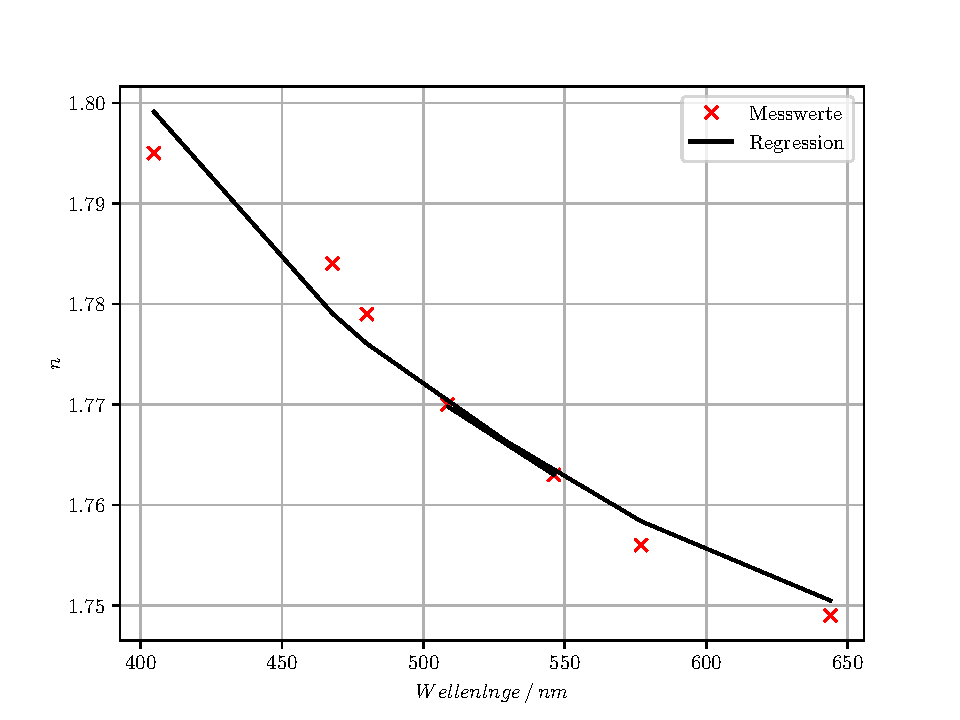
\includegraphics[width=\textwidth]{plot1.pdf}
  \caption{Darstellung der Dispersionskurve.}
  \label{abb:4}
\end{figure}
Die Regressionskurven sind jeweils mit der Gleichung \ref{eq:3} und \ref{eq:4} durchgeführt worden.
Es ergeben sich für die Parameter folgende Werte:
\begin{itemize}
  \item $A_0 = \SI{2.952(17)}{\per\nano\meter}$
  \item $A_2 = \SI{46604.06(409599)}{\per\nano\meter}$
  \item $A'_0 = \SI{3.322(020)}{\per\nano\meter}$
  \item $A'_2 = (6,771 \pm 0,703)10^{-7} \si{\per\nano\meter}$
\end{itemize}
Um nun bestimmen zu können, welche Annahme zur Dispersionskurve genommen werden soll, wird
die Methode der kleinsten Quadrate zunächst bestimmt.
\begin{equation*}
  s^2_n = \frac{1}{z-2} \sum_{i=1}^{z}(n^2(\lambda_i)-A_0-\frac{A_2}{\lambda^2_i})^2 \,\,\, \text{für} \, \lambda >> \lambda_1
  \label{eq:10}
\end{equation*}
\begin{equation*}
  s^2_{n'} = \frac{1}{z-2} \sum_{i=1}^{z}(n^2(\lambda_i)-A'_0+A'_2 \cdot \lambda^2_i)^2 \,\,\, \text{für} \, \lambda << \lambda_1
  \label{eq:11}
\end{equation*}
Die eingesetzten Werte ergeben aufsummiert.
\begin{itemize}
  \item $s^2_n = 0,2053$
  \item $s^2_{n'} = 0,0002$
\end{itemize}
Da $s^2$ möglichst klein sein soll, wird die Formel \ref{eq:4} für $\lambda << \lambda_1$ genutzt.
Es folgt für den Brechungsindex folgende Gleichung
\begin{equation}
  n(\lambda)= \sqrt{3,322 - 6,771\cdot 10^{-7} \cdot \lambda^2}.
  \label{eq:12}
\end{equation}

Mithilfe der Dispersionsgleichung \ref{eq:12} wird die \textbf{Abbesche Zahl} bestimmt.
Sie sagt aus wie die Farbzerstreuung von dem \textbf{SF15} ist.
Die Gleichungen lautet
\begin{equation}
  \nu = \frac{n_D -1}{n_f-n_c}.
  \label{eq:13}
\end{equation}
Mit Gleichung \ref{eq:12} werden die Ergebnisse in der Tabelle \ref{tab:3}
dargestellt. Für die Wellenlänge werden die Fraunhoferschen Linien verwendet.
\begin{table}[H]
  \centering
  \caption{Bestimmung der Brechungsindices mit den Fraunhoferschen Linien.}
  \label{tab:3}
  \begin{tabular}{c c c c }
    \toprule
    $\text{Linie}$ & $\text{Wellenlänge} \,/\,\si{\nano\meter}$ & $\text{Brechungsindex}$ &$n$\\
    \midrule
    $\lambda_c$ & 656 & 1,741 & $n_c$\\
    $\lambda_D$ & 589 & 1,757 & $n_D$\\
    $\lambda_F$ & 486 & 1,778 & $n_F$\\
    \bottomrule
  \end{tabular}
\end{table}
Mit Gleichung \ref{eq:13} lautet die \textbf{Abbesche Zahl}
\begin{equation*}
  \nu = 20,56
\end{equation*}

Für das Auflösungsvermögen werden zwei benachbarte Wellenlängen
als Wellenlängeunterschied $\Delta\lambda$ bezeichnet. Der Wellenlängeunterschied $\Delta\lambda$ muss
so gering sein, dass sie gerade vom Gerät getrennt werden können.
Der Ausdruck für das Auflösungsvermögen lautet
\begin{equation*}
  A = \frac{\lambda}{\Delta\lambda}
\end{equation*}
Durch Näherungen von Winkelfunktionen kann das Auflösungsvermögen umgeschrieben werden zu
\begin{equation}
  A = b \frac{d}{d\lambda} n(\lambda).
  \label{eq:14}
\end{equation}
Dabei ist $b$ die Basislänge vom Prisma und beträgt $\SI{3}{\centi\meter}$.
Nun wird die Gleichung \ref{eq:4} nach $\lambda$ abgeleitet und in die Gleichung \ref{eq:14}
eingesetzt.
Es folgt für das Auflösungsvermögen:
\begin{equation}
  A = b \cdot \frac{-6,771\cdot10^{-7} \lambda}{\sqrt{3,322 - 6,771\cdot10^{-7} \lambda^2}}
\end{equation}
Die Ergebnisse werden in der Tabelle \ref{tab:4} dargestellt.
\begin{table}[H]
  \centering
  \caption{Auflösungsvermögen von den Fraunhoferschen Linien.}
  \label{tab:4}
  \begin{tabular}{c c c}
    \toprule
    $\text{Linie}$ & $\text{Wellenlänge} \,/\,\si{\nano\meter}$ & $\text{Auflösungsvermögen}$\\
    \midrule
    $\lambda_c$ & 656 & 7654,42 \\
    $\lambda_D$ & 589 & 6809,48\\
    $\lambda_F$ & 486 & 5551,68\\
    \bottomrule
  \end{tabular}
\end{table}

Um nun die nächste abgelegene Absorptionstelle $\lambda_1$ zu bestimmen wird
mit der Lösung der Dispersionsgleichung ein Koeffizentenvergleich von $A'_0 \, ,\, A'_2$ gemacht.
Der Vergleich wird mit der Gleichung \ref{eq:4} durchgeführt.
Somit ergeben sich für 
\begin{equation*}
  A'_0 =
\end{equation*}
